%literature review
%photoshop
\subsection{Changing and matching skin colour in Photoshop}

Skin colour correction is a frequent problem encountered in photo retouching and there are a wide range of online video tutorials available documenting the methods artists use to manually adjust human skin tone in individual images using Adobe Photoshop, a widely used commercial image manipulation software. The purposes of these videos include giving the subject of an image the appearance of a tan, matching the skin tone of the subject to a desired skin tone on another individual, or matching the skin tone of a subject's face to the rest of the subject's body, which is often a slightly different colour \cite{photoshop:tan, photoshop:match_other, photoshop:match_body}. Bearing in mind that techniques described by such tutorials expect artistic input from a human editor to acheive the results and are therefore not entirely aligned with the purposes of this project, it is useful to study these methods because the results achieved are usually extremely realistic and aesthetically pleasing and should be a standard that the algorithm developed in this project strives towards. We therefore surveyed a number of these videos and summarize below the techniques of some of the most relevant videos.

\subsubsection*{Summary of Photoshop techniques}

Shaver demonstrated how to change a person's skin colour from dark to light \cite{photoshop:obama}, which is an impressively wide range to change. Shaver used levels and curves, which are tools that manipulate the $rgb$ colour histogram of the image, to increase brightness to an extent, then performed further brightening by using a grey scale conversion to brighten the skin area of a black and white image and then using the luminosity blend mode to place the colour back into the image. We show the results acheived in Table \ref{tab:obama_demo}.

\begin{longtable}{|c|c|}
    \caption{Screen captures from Photoshop tutorial for changing skin colour from dark to light. \label{tab:obama_demo}}\\
    \hline
    Original & Result \\
    \hline
  \begin{minipage}{.29\textwidth}
    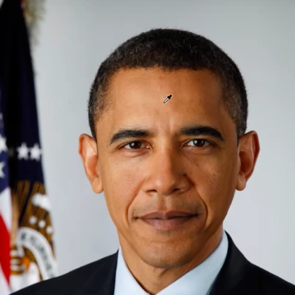
\includegraphics[width=\textwidth,height=\textheight,keepaspectratio]{images/obama_orig}
  \end{minipage} & 
  \begin{minipage}{.29\textwidth}
    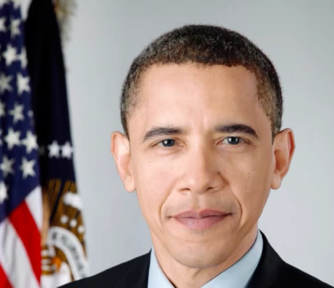
\includegraphics[width=\textwidth,height=\textheight,keepaspectratio]{images/obama_res}
  \end{minipage} \\
    \hline
\end{longtable}

Phlearn demonstrated an effect in the reverse direction by demonstrating a technique for giving the model the image appearance of a dark tan \cite{photoshop:tan}. The highlights and shadows of the image are adjusted separately by using the ``blend if" function of Photoshop, which blends in an effect only if the original pixel is above a certain threshold of brightness.

Phlearn also demonstrated a method for matching the skin colour of body and face in an image where the two appear mismatched \cite{photoshop:match_body}. The author sampled a range of colours from the body and adjusted the face with the levels tool for each colour channel. We show the results acheived in Table \ref{tab:match_body_demo}.

\begin{longtable}{|c|c|c|}
    \caption{Screen captures from Photoshop tutorial for matching the skintones of face and body. \label{tab:match_body_demo}}\\
    \hline
    Original & Target & Result \\
    \hline
  \begin{minipage}{.29\textwidth}
    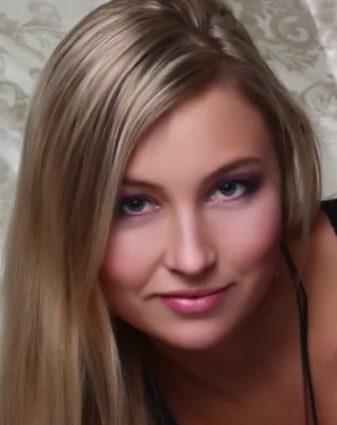
\includegraphics[width=\textwidth,height=\textheight,keepaspectratio]{images/match_body_orig}
  \end{minipage} & 
  \begin{minipage}{.29\textwidth}
    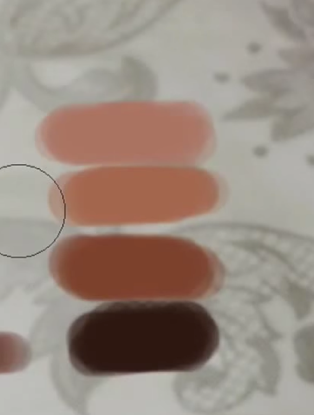
\includegraphics[width=\textwidth,height=\textheight,keepaspectratio]{images/match_body_targ}
  \end{minipage} & 
  \begin{minipage}{.29\textwidth}
    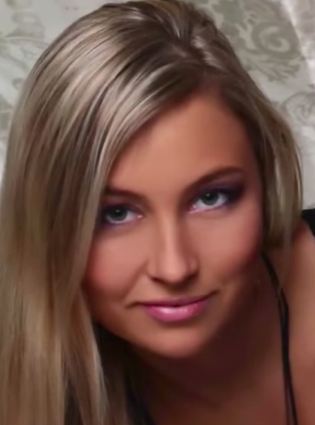
\includegraphics[width=\textwidth,height=\textheight,keepaspectratio]{images/match_body_res}
  \end{minipage} \\
    \hline
\end{longtable}

PiXimperfect demonstrated a method for matching skin colour in one portrait to another \cite{photoshop:match_other}. PiXimperfect first calculates the two average colours of the faces and uses the Photoshop curves tool to match the average colours of the original image to the target image. There must then be further adjustments by eye to change colour, brightness and contrast. Examples of the results from PiXimperfect is show in Table \ref{tab:match_other_demo}

\begin{longtable}{|N||c|c|c|}
    \caption{Screen captures from Photoshop tutorial for matching the skintones of portraits of different people. \label{tab:match_other_demo}}\\
    \hline
    \multicolumn{1}{|c||}{No.} & Original & Target & Result \\
    \hline  \label{row:photoshop_match_other_1} &
  \begin{minipage}{.29\textwidth}
    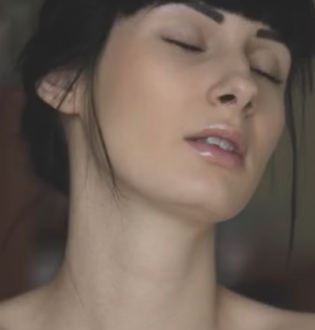
\includegraphics[width=\textwidth,height=\textheight,keepaspectratio]{images/match_other_1_orig}
  \end{minipage} & 
  \begin{minipage}{.29\textwidth}
    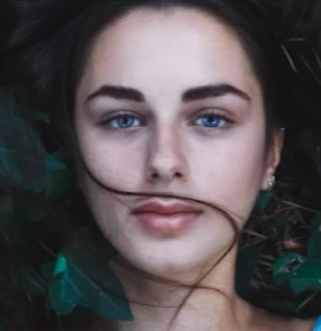
\includegraphics[width=\textwidth,height=\textheight,keepaspectratio]{images/match_other_1_targ}
  \end{minipage} & 
  \begin{minipage}{.29\textwidth}
    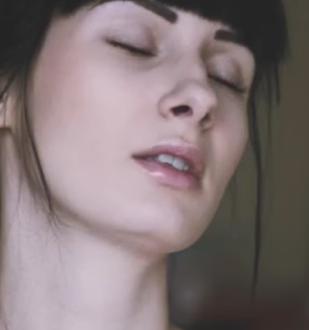
\includegraphics[width=\textwidth,height=\textheight,keepaspectratio]{images/match_other_1_res}
  \end{minipage} \\
    \hline  \label{row:photoshop_match_other_2} &
  \begin{minipage}{.29\textwidth}
    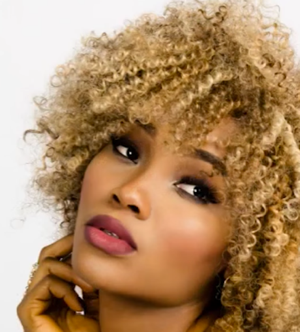
\includegraphics[width=\textwidth,height=\textheight,keepaspectratio]{images/match_other_2_orig}
  \end{minipage} & 
  \begin{minipage}{.29\textwidth}
    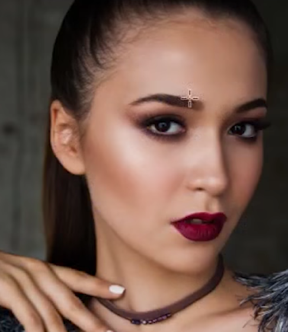
\includegraphics[width=\textwidth,height=\textheight,keepaspectratio]{images/match_other_2_targ}
  \end{minipage} & 
  \begin{minipage}{.29\textwidth}
    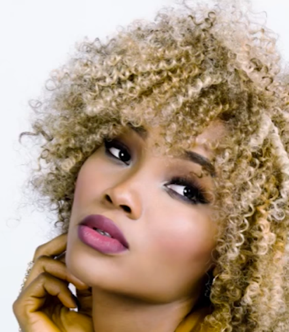
\includegraphics[width=\textwidth,height=\textheight,keepaspectratio]{images/match_other_2_res}
  \end{minipage} \\
    \hline
\end{longtable}

In summary, for most of the techniques surveyed, levels and curves are frequently used for small brightness adjustments \cite{photoshop:obama, photoshop:match_body, photoshop:match_other}, and often to reduce the vividness of the colour adjustments the saturation must be slightly decreased \cite{photoshop:obama, photoshop:match_body}. After all other effects are applied, the opacity of the overall effect is often reduced from 100\% for a more natural appearance \cite{photoshop:obama, photoshop:match_body}.

\subsubsection*{Limitations of Photoshop techniques}
Unlike the purpose of our project, the Photoshop techniques surveyed are not meant for automation. Instead, they are meant to be tailored to each specific image that a human is adjusting, and there are many junctures where the specific numerical amount of an adjustment often have to be judged by eye. While Photoshop has a method for automating processes using actions, the processes are meant for increasing ease of use by artists who can make additional adjustments and are familiar with the tool, rather than for use in commercial applications where the process is entirely automated \cite{photoshop:actions}.

Another limitation is that Photoshop operates at a higher level of abstraction than image processing software making use of libraries such as OpenCV. Image processing code has much more control over processes that can be applied to images, and the regions on the image that processes are applied to. 

Finally, some Photoshop effects may be proprietary and are of course limited to the platforms that Photoshop supports, while a program developed with a platform such as OpenCV can be made open source and adapted to uses on a variety of different platforms.

\subsection{Academic work related to colour transfer and skin colour enhancement \label{sec:academic_work}}

We have also surveyed the current state of the academic work relevant to our project, which fall into four rough categories:

\textbf{Colour transfer for general images.} There is a large body of work on the subject of automatically transferring the ``style" or colours in an example image to another image. The work in this area is focused on being effective for a wide range of colours in general images, not necessarily skin colour; however, skin colour transfer algorithms and processes often refer to this body of work and so this area is of interest to us.

\textbf{Colour transfer for human skin colour.} There have also been several prior studies transferring colour specifically for images wherein skin colour is prominent. These are most similar in purpose to our project and we will discuss each study in detail.

\textbf{Skin colour transfer as part of other applications.} We have also found several examples of practical application of skin transfer algorithms, where the practical use of usually a relatively simple skin transfer algorithm is demonstrated as part of a larger project. 

\textbf{Skin colour enhancement mobile applications.} Finally, there is the related field of skin tone enhancement software, where algorithms are usually intended to adjust the user skin colour towards a more pleasing tone and not to a specific target colour. We include the this field because unlike the other categories of prior work there are several studies of adjusting skin tone on a mobile device, which is part of the requirements for this project.

\subsubsection{Colour transfer by example image for general images}
Colour transfer refers to modifying the colours of an image (the \textit{source image}) to give it the desired appearance and style demonstrated by an example image, which we will refer to as the \textit{target image}. Table \ref{tab:reinhard_demo} illustrates an example of this effect.

There have been a wide range of studies done in this area beginning with the seminal work of Reinhard et al. in 2001 \cite{reinhard_2001_transfer}. The authors first convert the image into $l\alpha\beta$ colour space, a colour space designed for natural scenes and based on research into human perception to reduce the correlation between each channel and remove the need to consider cross-channel effects when performing transformations on each channel. The authors then perform a simple operation to match the average and standard deviation of each channel of the original image to that of the target image. The resultant image is then converted back into $RGB$ space.
%in this paper we replicate this method for comparison purposes?

\begin{table}[H]
    \centering
    \caption{Example of image colour transfer using the algorithm from Reinhard et al. All images from \cite{reinhard_2001_transfer} \label{tab:reinhard_demo}}
\begin{tabular}{|c|c|c|}
    \hline
    Source & Target & Output \\
    \hline
  \begin{minipage}{.29\textwidth}
    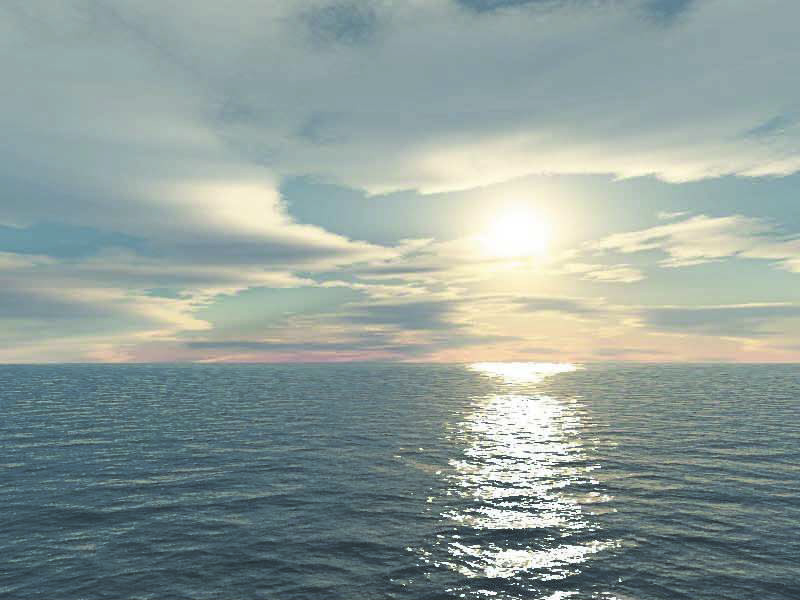
\includegraphics[width=\textwidth,height=\textheight,keepaspectratio]{images/reinhard_orig1}
  \end{minipage} & 
  \begin{minipage}{.29\textwidth}
    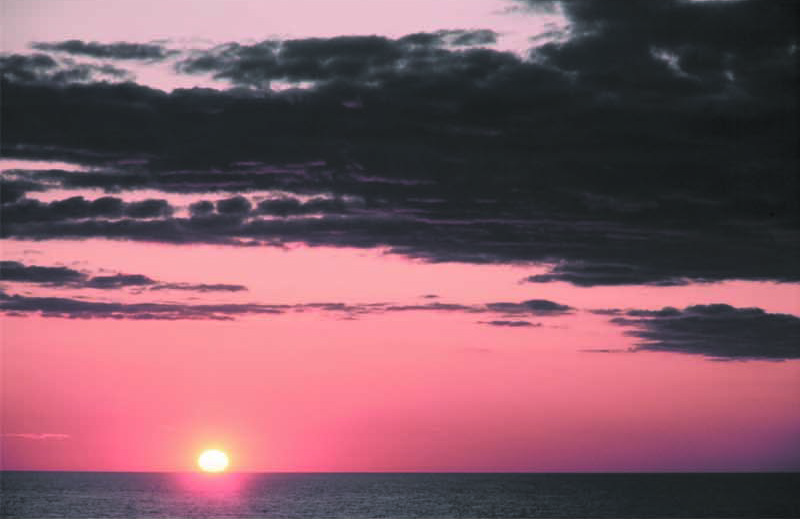
\includegraphics[width=\textwidth,height=\textheight,keepaspectratio]{images/reinhard_target1}
  \end{minipage} & 
  \begin{minipage}{.29\textwidth}
    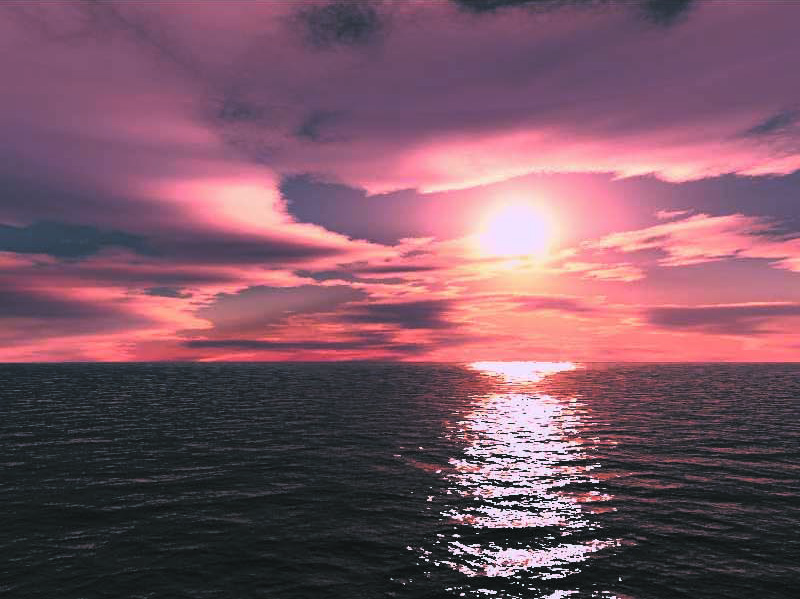
\includegraphics[width=\textwidth,height=\textheight,keepaspectratio]{images/reinhard_result1}
  \end{minipage} \\
    \hline
\end{tabular}
\end{table}

In a later study, Piti\'{e} et al. developed a method for entirely transferring the exact statistical distribution of the colours of the target image to the original image \cite{pitie_2005_pdf}, and later improved on the technique with the motivation of automating film grading, or the process of enhancing frames in films to ensure consistency of colour and mood \cite{pitie_2007_grading}. We show an example the effects they achieve in Table \ref{tab:pitie_demo}

\begin{table}[H]
    \centering
    \caption{Example of film grading based on an example image using the algorithm from Piti\'{e} et al. All images from \cite{pitie_2007_grading} \label{tab:pitie_demo}}
\begin{tabular}{|c|c|c|}
    \hline
    Source & Target & Output \\
    \hline
  \begin{minipage}{.29\textwidth}
    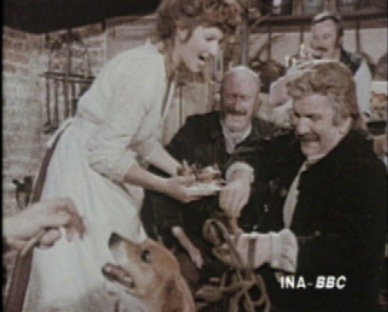
\includegraphics[width=\textwidth,height=\textheight,keepaspectratio]{images/pitie_original}
  \end{minipage} & 
  \begin{minipage}{.29\textwidth}
    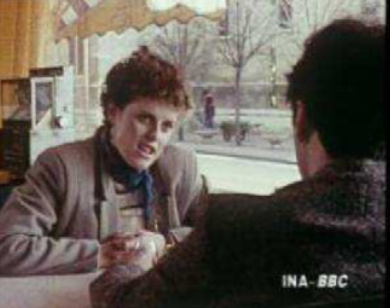
\includegraphics[width=\textwidth,height=\textheight,keepaspectratio]{images/pitie_target1}
  \end{minipage} & 
  \begin{minipage}{.29\textwidth}
    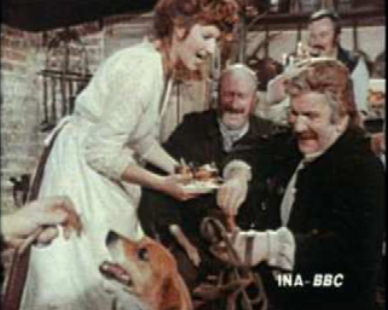
\includegraphics[width=\textwidth,height=\textheight,keepaspectratio]{images/pitie_result1}
  \end{minipage} \\
    \hline
  \begin{minipage}{.29\textwidth}
    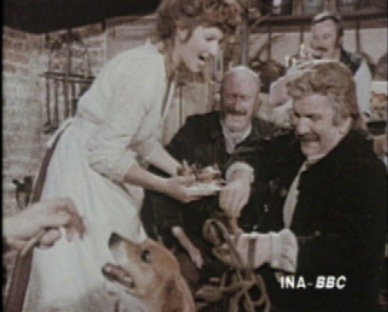
\includegraphics[width=\textwidth,height=\textheight,keepaspectratio]{images/pitie_original}
  \end{minipage} & 
  \begin{minipage}{.29\textwidth}
    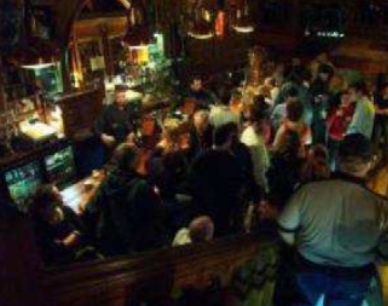
\includegraphics[width=\textwidth,height=\textheight,keepaspectratio]{images/pitie_target2}
  \end{minipage} & 
  \begin{minipage}{.29\textwidth}
    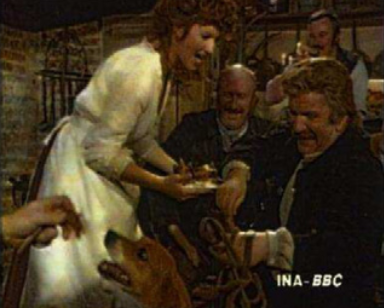
\includegraphics[width=\textwidth,height=\textheight,keepaspectratio]{images/pitie_result2}
  \end{minipage} \\
    \hline
\end{tabular}
\end{table}
%in this paper we replicate this method based on code found online?

More recently, Bonnel et al. conducted a further study on colour transfer for film grading considering both spacial and temporal information \cite{bonneel_2013_video} and Chang et al. created a tool for user editing of an image based on a automatically generated colour palette \cite{chang_2015_palette}.

While these techniques are interesting possibilities to try when transferring human skin colour, because these prior studies are all concerned with different problems that can arise with general images but not specifically for human skin colour, studies that specifically relate to human skin colour demonstrate that the general colour transfer techniques can be improved upon.

\subsubsection{Colour transfer by example for images with human skin}
There are fewer studies done specifically on the transfer of human skin colour, but there are several of great interest to us.

Seo et al. has a purpose most similar to the purpose of this project, which is to find a method of transferring human skin colours as realistically and accurately as possible \cite{seo_2005_transfer}. In their study, authors demonstrate results that improve in realistic appearance compared to the Reinhard's algorithm. To achieve this, authors model the skin colour as an elongated distribution around a line referred to as the \textit{principle line} in $RGB$ space. To perform the colour transfer, the authors transform the distribution of the original image such that the principle line aligns with that of the target image. The authors then break the colour values into bins along the principle lines and also match the distribution of each bin. Table \ref{tab:seo_demo} demonstrates the output of this method.

\begin{table}[H]
    \centering
    \caption{Example of image colour transfer using the algorithm from Seo et al. All images from \cite{seo_2005_transfer} \label{tab:seo_demo}}
\begin{tabular}{|c|c|c|}
    \hline
    Source & Target & Output \\
    \hline
  \begin{minipage}{.29\textwidth}
    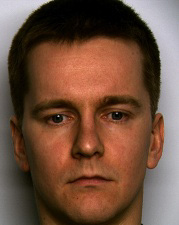
\includegraphics[width=\textwidth,height=\textheight,keepaspectratio]{images/seo_orig1}
  \end{minipage} & 
  \begin{minipage}{.29\textwidth}
    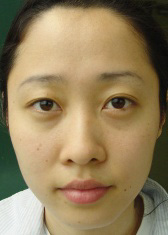
\includegraphics[width=\textwidth,height=\textheight,keepaspectratio]{images/seo_target1}
  \end{minipage} & 
  \begin{minipage}{.29\textwidth}
    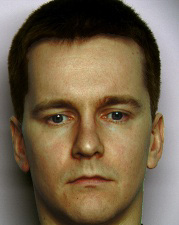
\includegraphics[width=\textwidth,height=\textheight,keepaspectratio]{images/seo_result1}
  \end{minipage} \\
    \hline
\end{tabular}
\end{table}

However, as far as the requirements of this project is concerned, it is not clear how fast this algorithm can run, particularly on a mobile device, nor the range of colours that the algorithm can realistically transform between, and it is in these areas that our project will attempt to improve upon.
% should we possibly replicate and check?

Yang et al. performed a more recent study of colour transfer for human portraits \cite{yang_2017_semantic} - Table \ref{tab:yang_demo} demonstrates their results. However, as Table \ref{tab:yang_demo} shows, this study focuses on the effect on the whole portrait, and places emphasis on transferring colour for different features of the human face. The actual algorithm the authors use to transfer skin colour is actually Reinhard's algorithm. This method also ranks the preferred target image for similarity to the source image before performing the colour transfer, which differs from our project where a key issue is that we have no control over the target image that the user will provide us and must be able to transfer to a wide range of colours. 

\begin{table}[H]
    \centering
    \caption{Example of image colour transfer using the algorithm from Yang et al. All images from \cite{yang_2017_semantic} \label{tab:yang_demo}}
\begin{tabular}{|c|c|c|}
    \hline
    Source & Target & Output \\
    \hline
  \begin{minipage}{.29\textwidth}
    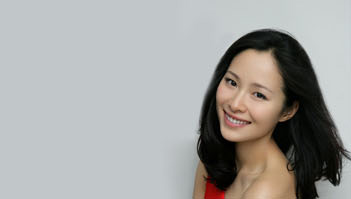
\includegraphics[width=\textwidth,height=\textheight,keepaspectratio]{images/yang_orig1}
  \end{minipage} & 
  \begin{minipage}{.29\textwidth}
    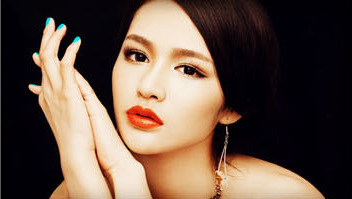
\includegraphics[width=\textwidth,height=\textheight,keepaspectratio]{images/yang_target1}
  \end{minipage} & 
  \begin{minipage}{.29\textwidth}
    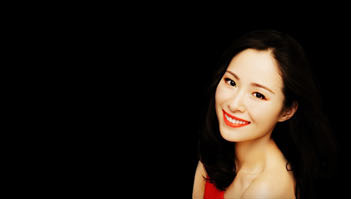
\includegraphics[width=\textwidth,height=\textheight,keepaspectratio]{images/yang_result1}
  \end{minipage} \\
    \hline
\end{tabular}
\end{table}

Yin et al. performed a study on the transfer of skin colour between races in order to aid a psychological study \cite{yin_2004_transfer}. The authors use a process of first global adjustment of the two images to match the average colours, and then using the pixels from the target image with a colour most resembling the colour in the source image to entirely replace that pixel in the source image. Table \ref{tab:yin_demo} shows an example of the results using this technique.

\begin{table}[H]
    \centering
    \caption{Example of image colour transfer using the algorithm from Yin et al. All images from \cite{yin_2004_transfer} \label{tab:yin_demo}}    
\begin{tabular}{|c|c|c|}
    \hline
    Source & Target & Output \\
    \hline
  \begin{minipage}{.29\textwidth}
    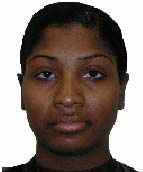
\includegraphics[width=\textwidth,height=\textheight,keepaspectratio]{images/yin_orig1}
  \end{minipage} & 
  \begin{minipage}{.29\textwidth}
    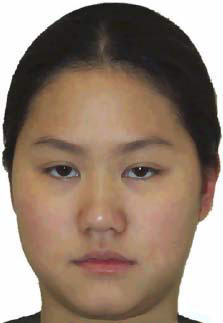
\includegraphics[width=\textwidth,height=\textheight,keepaspectratio]{images/yin_target1}
  \end{minipage} & 
  \begin{minipage}{.29\textwidth}
    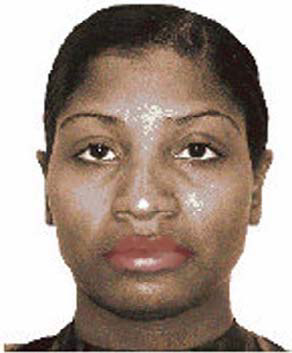
\includegraphics[width=\textwidth,height=\textheight,keepaspectratio]{images/yin_result1}
  \end{minipage} \\
    \hline
\end{tabular}
\end{table}

We include this study because it is one of the few that explicitly tries to transfer colour between large difference of skin colour, however, we feel it has many flaws with respect to our requirements. Particularly in the case of large skin colour changes shown above, the results are not realistic and show bright spots of saturation. Furthermore, the authors describe their algorithm as having $O(n^2)$ time, which likely means that this algorithm will perform too slowly for our purposes.

% quality of transfer - bright spots, realism for transfer from a lighter or midtoned skin colour to darker skin colour, and time taken to perform the transfer


\subsubsection{Skin colour transfer as part of other applications}
Several applications performing different functions make use of skin colour transfer.

Shilkrot et al. published a study on transferring the identity of the user on to a model image wearing garments the user may desire to purchase to create the virtual experience of the user trying on the garment \cite{shilkrot_2013_garment}. The purpose of this article is fundamentally related to the purpose of the application that is this project's goal to support, and so this article is of great interest to us. In fact, as part of the identity transfer, this article performs skin colour transfer on the model image to take on the skin colour of the user. Shilkrot uses a Gaussian Mixed Model for transfer skin colours and seems to use it for a relatively wide range of colour differences.
%explain this model
%Is there user interaction?
%timing wise, how fast?
%include figures of results

The difference between Shilkrot's study and ours is that skin is only a small part of their final image, and the skin transfer process is only a small part of their study, which also places emphasis on the transfer of the user's head and the reshaping of the model's body proportions. In our case, the hand will be the only object of interest in our inputs and outputs. While we need not devote our efforts to any aspect but the skin colour change, any flaws in the colour transfer causing unrealistic results will be much more noticeable. 
% Are there other identity transfer articles?

Another interesting case of skin colour matching is the work of Bitouk et al to create a face swapping software that seamlessly changes faces in photos to stock photo faces \cite{bitouk_2008_faceswap}. Since the skin colour of a stock photo face would never exactly match the rest of the skin colour in the original photo, the authors adjust the lighting and skin colour until they do match. However, the authors specifically state that large skin colour changes cannot be made, and to support a wide range of skin colours, the authors rely on having a large library of stock photos of every lighting position and skin colour. On the other hand, for our project, we are motivated by that fact that it is difficult to prepare videos for the full range of user skin colours.
%but it's fast though, should mention that

Another application we've found is the work of Baba et al. to develop a software that edits portraits in yearbook photos to all have a uniform skin colour given an example skin colour image \cite{baba_2015_yearbook}. The algorithm that the authors use to achieve this uses Pitié's colour grading algorithm and guided image filtering. However, the goal of the project in terms of skin colour appears to be to have skin colours close to the target image but not necessarily exactly the same; the authors are focusing on the overall appearance of the set of portraits rather than the accuracy of the skin colour transfer for each individual image. On the other hand, the goal of our project is to ensure that the transformed skin colour of the model is as accurate as possible to the user's skin colour.
%explain guided image filtering

\subsubsection{Skin colour enhancement mobile applications}
For the most part the studies we have found are not meant to be run on a mobile platform and there are few studies specifically pertaining to human skin colour. There are, however, many skin colour enhancement applications that modify human skin colour and several studies that perform this on mobile devices.

%This makes sense as mobile devices all have cameras and these days skin tone enhancement is part of the functionality of the camera
%exceptions though - which algorithms are fast? garment,
%are you sure there are no other skin color change stuff on mobile platform? look more into this
%Mention the 2 studies at least
For example, Lee et al. enhances skin colour of users to a \textit{preferred skin colour}, or a skin colour close to the user's original skin colour that a member of the user's ethnic group would find the most pleasing, in addition to changing the background of the user's video on a mobile phone \cite{lee_2010_mobile}. They perform the skin colour transformation in $HSV$ or hue, saturation and value colour space, simply adding the difference between the average hue and saturation values between the image and the target colour, damping the offset they add by a multiplicative factor for more realistic-appearing results. 
% ?? We show an example of their results in Table \ref{}

The difference in purpose between such studies and ours is that we have a specific target colour that could be different from the aesthetically pleasing colour that skin enhancement is aiming for, and our requirements for accuracy to the target colour is more stringent.

\subsection{Summary of differences between prior studies and this project}

In summary, we find that the prior work can satisfy some but not all of our requirements for this project. Most of the sophisticated colour transfer work done is for general images and not meant to accurately and realistically transfer human skin colour. On the other hand, much of the work done related to correcting human skin colour is meant to improve the subjective appearance of human skin, and not meant to accurately change the human skin colour to a specific shade. For studies specifically addressing the recolouring of human skin, many of the techniques are not meant to achieve skin colour transfer between a large difference in skin colour. The study we found that did perform transforms across a large range often did not have sufficiently convincing and artifact-free results. Finally, most of the results we surveyed do not perform the transformation at a speed fast enough for a mobile application, or else have not given the speed of the algorithm significant consideration. We will attempt to address all these areas in our project.
%explain theoretical concepts in context of thesis work; be clear and concise
%summarize relevant research to give understanding of current field
%analyze research in field to give deeper understanding of research question 
%indicate a path going forward
